\documentclass{article}

\usepackage[utf8]{inputenc}
\date{}
\usepackage{amsthm,amssymb,amsmath}
\usepackage{graphicx}
\graphicspath{ {./images/} }



\newcommand{\NN}{\mathbb{N}}
\newcommand{\ZZ}{\mathbb{Z}}
\newcommand{\RR}{\mathbb{R}}
\newcommand{\QQ}{\mathbb{Q}}
\newcommand{\CC}{\mathbb{C}}
\newtheorem{theorem}{Theorem}[section]
\newtheorem{corollary}{Corollary}[theorem]
\newtheorem{lemma}[theorem]{Lemma}
\newtheorem{proposition}[theorem]{Proposition}
\newtheorem{conjecture}{Conjecture}
\newtheorem{definition}{Definition}
\theoremstyle{remark}
\newtheorem{example}{Example}
\newtheorem{answer}{Answer}
\newtheorem{remark}[example]{Remark}

\title{ODE with Lipschitz Coefficients Draft 2}
\author{Phillip Yan}


\begin{document}

\maketitle

%%%%%%%%%%%%%%%%%%%%%%%%%%%%%%%%%%%%%%%%%%%%%%%%%%%%%%%%%%%%%%%%%%%%%%%%%%%%%%


\section{Introduction to ODEs}

\subsection{Solving ODEs and Examples}

A key concept in math that appears often in the real world is the idea that sometimes for equations, it is easier to consider the rate of change rather than the absolute amount of change.

A clear real world example can be seen in the expression of acceleration as the change in velocity. That is, 

$$v'(t) = a(t),$$

\noindent where $v'(t)$ is the change in velocity at a given moment of time t, and $a(t)$ is a function for acceleration at time $t$. Here, in the absence of a clear velocity function, we see the change of velocity expressed as a function of acceleration. Similarly within physics, it is possible to model the motion of a pendulum with the following equation.
Consider $\theta(t)$ for the angular displacement of the pendulum as a function of time, $L$ for the length of the string, and $g$ as the constant for acceleration due to gravity. Then $\theta$ and its derivatives satisfy the following equation and image: \\


$$\frac{d^2\theta}{dt^2}  = - \frac{g}{L}\sin{\theta}.$$

\begin{center}\includegraphics[width=3cm]{Pendulum.png} \\ A free body diagram of a pendulum with a leftward facing  arrow corresponding to $\frac{d^2\theta}{dt^2}$, or the rate of change of the rate of change given the pendulum's current angular displacement. \end{center}

Note that an explicit formula for $\theta(t)$ is not known. Instead, we only that it satisfies the equation above which is derived from principles in physics.

Both of these equations are examples of differential equations which are defined as the following.
\begin{definition} A \textbf{differential equation} is an equation containing the derivatives of one or more unknown functions with respect to one or more independent variables.
\end{definition}

The equation for pendulum displacement is an example of a differential equation where the unknown function is $\theta$ and the independent variable time $t$.

An example of a differential equation where there are multiple independent variables is the heat equation in physics which models the diffusion of heat,
$$\frac{\partial u}{\partial t} = k\frac{\partial^2 u}{\partial x^2}$$
\noindent where $u$ is the temperature, $x$ a given point in space, and $k$ is the thermal diffusivity of the material. Intuitively, this equation describes the rate of change of temperature over time at a given point in space and time based on the derivative of the rate of change of temperature as you move from point $x$ in space.

There are many different types of differential equations. A special kind of differential equation that will be the focus of this paper is the Ordinary Differential Equation.

\begin{definition}
\textbf{An ordinary differential equation (ODE)} is 
    a differential equation that contains derivatives with respect to a single independent variable.
\end{definition}



For this paper, we  will consider \textbf{first-order ODEs}, which are ODEs of the form
$$y'(x) = f(x,y)$$
\noindent for some function $f: \Bbb R^2 \to \Bbb R$.

Intuitively, like all differential equations, an ODE is a representation of a rate of change. In this particular case, the derivative of a function, $y'(x)$, is expressed in terms of a function of $x$ and $y$ itself. \\


A classic example of an ODE is the \textbf{Lotka-Volterra} predator-prey model in systems biology which is a pair of ODEs used to model the relationship between the population of a predator and the population of a prey. The two equations $\frac{dx}{dt}$ and $\frac{dy}{dt}$ represent the population growth rate of the prey and predator, respectively, at a given moment in time. The equations are

$$\frac{dx}{dt} = \alpha x - \beta xy$$
$$\frac{dy}{dt} = \delta xy - \gamma y$$

\noindent where $x$ is the population density of the prey, $y$ the population density of the predator. Each equation has parameters, with the prey's parameters $\alpha$ and $\beta$ describing respectively the natural per capita growth rate of the prey and a scaling factor to describe the impact of predation on the $\alpha x$ natural growth rate. For predators, $\delta$ and $\gamma$ describe respectively the impact of the presence of prey on the predator growth rate and the natural death rate of the predator. Taken together, this straightforward model can be used as a basis to model the impact of the presence of a predator and its prey on the overall rate of change in the population density of the two species. \\

For ODEs, because a function relating the dependent variable, $y$, with $x$ is not made explicit, one may wish to ``solve" the ODE, or to find the unknown function(s) of $y=f(x)$. By integrating an ODE of the form $y'(t) = f(t)$, we know from calculus that one obtains $y(x) = \int_0^t f(t) dt + C$, where $C$ is some constant value. This  gives us a family of functions for $y(t)$, which we can narrow down to a single function for $y(t)$ by choosing what $y(0) = C$ is from the start.\\
\begin{example}
In the acceleration example above, if one is given a starting velocity at time 0, $v(0) = 5m/s$, one can integrate both sides to obtain:

$$v(t) = \int_0^ta(s)ds + C.$$
Given $ v(0) = C = 5$, we get our specific solution:

$$v(t) = \int_0^ta(s)ds + 5.$$
Note that this satisfies the initial value $v(0) = 5m/s$. 

\end{example}

This is an example of an \textbf{initial value problem} which consists of an ODE alongside an initial value $(x_0, y_0)$ such that $y(x_0) = y_0$. The goal is to try to find a specific solution $y(x)$ which satisfies  both the ODE and the given initial value $y_0 = y(x_0)$.  \\


For example, returning to our pendulum example, an initial value might be $\theta(0) = \pi$, meaning the angular displacement at time 0 is $\pi$. Thus, we can intuitively reason that a different initial value can result in a different $\theta$ function. In this case, dropping a pendulum at different angular displacements can impact the resulting solution which is the function that relates angular displacement with time elapsed. \\



The process of integrating both sides to solve the ODE in Example 1 is called \textbf{direct integration}. When one can separate variables in the given equation, it is also possible to use a more complex method of solving ODEs called \textbf{separation of variables}. 

\begin{example}
Given an ODE which defines $y'$ in terms of both $y$ and $x$ values for some ODE,

$$ \frac{dy}{dx} = 10xy, \quad y(0) = 1$$

we can solve this with separation of variables because we can isolate the two variables on either side of the equation. Before we can divide both sides by y, though, we need to consider if there is a chance that $y=0$. In this case, note that the ODE becomes:
$$\frac{dy}{dx} = 10x(0) = 0 \implies y(x) = C.$$
Note that given $y(0) = 1,$ we know that therefore $C = 1$. Thus, note that in this case, $y$ can never be equal to 0, which results in a contradiction. Thus, now that we know $y \neq 0$, we can proceed with separation of variables.

Refactoring the expression to
$$  \frac{dy}{y} = 10xdx,$$

we can take the integral of both sides to solve the ODE:

\begin{align*}
\frac{dy}{y} &= 10xdx\\
\ln |y|  &= 5x^2 + C\\
|y| &= e^{5x^2 + C} \\
\end{align*}


We can address the absolute value by doing casework. Note that we can rule out the case when $y=0$ as we have shown that $y$ can never be equal to 0.

\begin{align*}
y<0 \implies y &= e^{5x^2 + C} \ \ = e^Ce^{5x^2}\\
y>0 \implies  y &= -e^{5x^2 + C} = -e^C e^{5x^2}\\
\end{align*}
Note that given our initial value $y(0) = 1$, we know that the following must be true for our first case:

$$y = e^Ce^{5x^2} \implies C = 0.$$

However, there does not exist a value C such that $-e^C e^{5x^2} = 1$, since $e^K > 0, \forall K \in R$. Thus, we have our specific solution when $y>0$.

\end{example}
\subsection{Existence}
Although there are many other methods to solve ODEs, as ODEs get more complex, the solution might not be immediately obvious. Sometimes they might not even exist. 

\begin{example}
An example of an ODE where the solution does not exist is 
$$ y'(x) = \begin{cases} 
      \frac{1}{x} & x \neq 0 \\
      0 & x= 0 \\
   \end{cases} , \quad y(0) = 0.$$

In order to have a solution $y$ for an ODE, note that $y'(x)$ must exist for all $x$ and that it must be equal to the given ODE. Consider the point $x = 0$. If we assume $y$ is differentiable at 0, then we know  $y'(0) = 0$ and that $y$ would be continuous at 0. However, considering values $x > 0$ and attempting to evaluate via direct integration 
we obtain the equation $$y(x) = \ln x + C.$$ Note that as $x \to 0^+$ from the right hand side, we have $\ln(x) \to -\infty$; in particular, $y(x)$ does not converge as $x$ goes to zero, so cannot be continuous at zero.

Therefore, because $x$ does not converge to 0, $y$ is not continuous at 0, meaning that there does not exist a differentiable function $y$ such that $y$ satisfies the ODE and the initial condition. 

Indeed, there exists a Cauchy-Peano Existence Theorem which tells us that if  $y'(x)$ is  continuous, then the ODE has at least one solutions. We will formally state this theorem in Section 4.2.
\end{example}

\subsection{Uniqueness}
At the same time, it is important to determine whether solutions are unique given a specific initial condition. In other words, we want to make sure that there is no randomness in output (the solutions) given a repeated input (the ODE). This is important in fields like physics which are deterministic. Returning again to our velocity and acceleration example, we wouldn't want two different velocity functions as our solution for the ODE and initial value problem. (You might end up with two different velocity values at a given time with the exact same acceleration and starting velocity, meaning you'll never know for certain what the  velocity is at any given moment!) \\

\begin{example} An example of an ODE where the solution is not unique is:

$$y'(x) = \sqrt{|y|}, \quad y(0) = 0.$$


Let us consider the two cases where $y>0$ and where $y<0$.

\textbf{Case 1 $(y>0)$}:
Evaluating this ODE via separation of variables and then direct integration, we see
\begin{align*}
y^{-\frac{1}{2}}\frac{dy}{dx} &= 1 \\
\int y^{-\frac{1}{2}}dy &= \int dx \\
2y^{\frac{1}{2}} &= x +C.
\end{align*}

Since we know via the initial value that $y(0) = 0$, we know that $C = 0$.

Thus, a solution is $y = \frac{x^2}{4}$.\\


\textbf{Case 2 $(y<0)$}:
Following the same process, except for $-y$, we get:
$$ 2(-y^{\frac{1}{2}}) = x.$$
Thus another solution is $y = -\frac{x^2}{4}$.




Furthermore, note that the tautological function $y = 0$ also is a solution. Although the solution to this same ODE but with a different initial condition might be unique, with the specific initial condition set by this initial value problem, $y(0) = 0$, there are three potential solution functions that satisfy the IVP.


We have the opposite problem as the previous ODE which had no solutions. This paper seeks to address the conditions that need to be satisfied so that there is exactly one solution.

\end{example}

\subsection{Example ODE With a Unique Solution}
Consider the ODE:
$$y'(x)= y^2 + xy + x^2, \quad y(0) = 0.$$

As a slightly more complex differential equation, it is not immediately obvious whether a solution exists and if that solution is unique. One can't easily separate the variables and directly integrate. Thus, for differential equations like these, we need some general theorem to assert that a solution exists and is unique.\\

In fact, we will see that this is a solvable ODE with a unique solution.


\subsection{Graphical Intuition}
Graphical intuition on the $xy$-plane might be helpful for our following discussion. Instead of a traditional graph of a function $y = f(x)$ which maps values of $x$ to values of $y$, we consider a slope field on the $xy$-plane. At every point $(x,y)$, the slope $\frac{dy}{dx}$ is calculated as a function of $x$ and $y$ and plotted on the graph to produce a field of different ``slopes" at all points in the graph. 

\begin{center}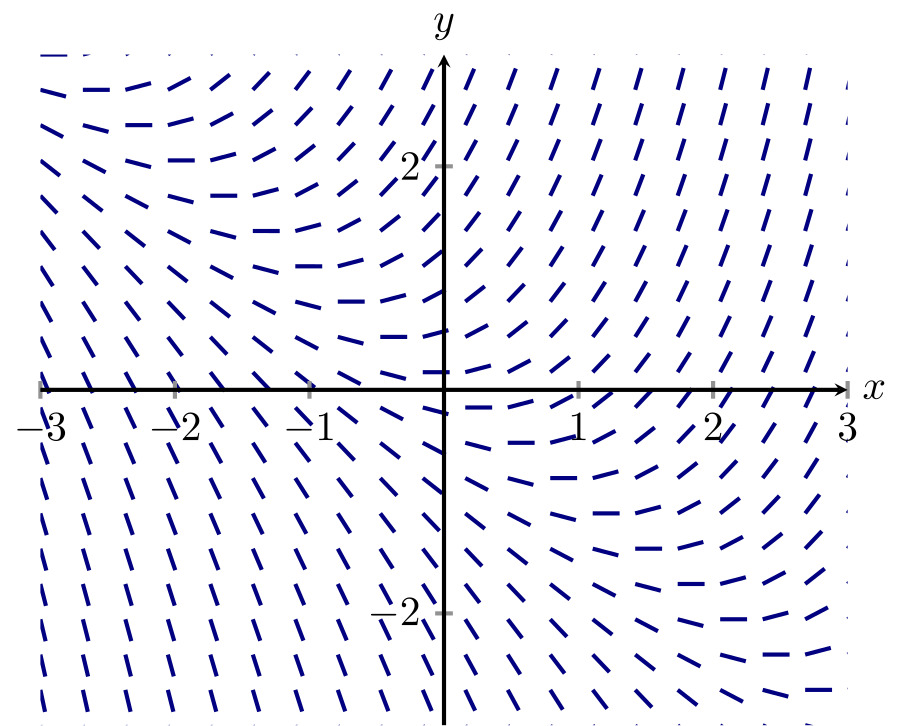
\includegraphics[width=7cm]{SlopeFieldMath.png} \\ A slope field for section 1.4 ODE ($y'(x)= y^2 + xy + x^2, y(0) = 0$) with the solution to the  initial value problem overlaid. \end{center}


Intuitively, when considering an initial value problem, one can potentially consider the initial coordinate pair as the coordinates of a boat, and the slope at any given point a current. Moving in the direction of the current, the ``boat" traces out a curve which is the function that is the solution if it exists to the ODE. \\


This intuition can help to serve as the basis to understand our approach in the following sections as it provides a visual basis for understanding the function $y'(x) = f(x,y(x)) + y_0$.



\section{Lipschitz Continuity}
In this paper, we will prove that such solutions exist locally and are locally unique given that the ODE is Lipschitz continuous on a specified set.

Our first step in understanding when solutions exist and are unique in ODEs is to introduce a stronger form of continuity than our previous epsilon-delta definition of general continuity.

We first introduce the concept of \textbf{metric spaces}, of which $\mathbb{R}$ is an example that we have used in class. \\

\begin{definition}
 A \textbf{metric space} $(X, d_X)$ is a set $(X)$ with a function $(d_X)$ defined as:

$$d_X: X \times X \to \Bbb [0, \infty )$$

such that $d_X$ satisfies the following three axioms given $x_1, x_2, x_3 \in X$:

\end{definition}
\begin{align*}
1.& \quad \text{The distance from a point to itself is 0: }d_X(x_1, x_1) = 0 \\ 
2.& \quad \text{Symmetry: } d_X(x_1, x_2) = d_X(x_2, x_1)\\
3.& \quad \text{The Triangle Inequality: }d_X(x_1, x_3) \leq  d_X(x_1, x_2) + d_X(x_2, x_3).
\end{align*}
\begin{example}
An example is the real vector space $\mathbb{R}^3$ equipped with absolute difference as the distance function: $d(x,y) = \|x-y\|$. It is straightforward to confirm that the absolute difference meets the above requirements for the distance function in a metric space given our understanding of absolute value on a number line.
\end{example}


We now can now define Lipschitz continuity: \\ 

\begin{definition} 
Given two metric spaces $(X, d_X)$ and $(Y, x_Y)$, a function $f: X \to Y$ is considered \textbf{Lipschitz continuous} if there exists $K \in [0, \infty)$ such that for all $x_1, x_2 \in X$,
$$d_Y(f(x_1),f(x_2)) \leq Kd_X(x_1,x_2).$$
\end{definition} 

Intuitively, a function is Lipschitz continuous over a certain interval if there exists a set constant value $K$ that bounds the magnitude of the derivative at any point within the interval. Visually, at every point there exists a ``double triangle" made from the two lines $y = K$ and $y = -K$ such that  the graph remains outside the triangle.\\

\begin{center}\includegraphics[width=7cm]{LipschitzContinuity.png} \\ A visual representation of the ``double" triangles used to determine Lipschitz continuity at the point $x = 0.5$. Note that the absence of the curve in the white triangles represents the fact that the derivative at 0.5 is bounded by K. \end{center}
\begin{example}
A clear example of a function that is Lipschitz continuous is $f: X \to Y, f(x) = x$. With the distance functions of the two metric spaces $(X = \Bbb R, d_X)$ and $(Y = \Bbb R, d_Y)$ both being the absolute difference, given two points $x_1, x_2 \in X$:
$$d_X(x_1 - x_2) = |x_1 - x_2| = |f(x_1) - f(x_2)|.$$

Thus, we know given any $K \geq 1$, $ |f(x_1) - f(x_2)| \leq K|x_1 - x_2|$ which satisfies the requirements of Lipschitz continuity.
\end{example}

\begin{example} 
A counter example can be seen in the function $f: X \to Y,  f(x) = \sqrt{|x|}$ on $x\in \Bbb R$. Let us refactor our definition of Lipschitz continuous to: 

$$ \frac{d_Y(f(x_1), f(x_2))}{d_X(x_1, x_2)} \leq K.$$

 Setting $x_1 = 0$ and given the absolute difference as the distance function, we see that this is the same as

$$ \frac{|\sqrt{|x_2|} - 0|}{|x_2 - 0|} \leq K.$$

In order for this function to be Lipschitz continuous, the above must be true for all $x_2 \in \Bbb R $. However, note that as $x_2$ approaches 0 from the right hand side, the following occurs:

$$\lim_{x_2 \to 0^+}\frac{|\sqrt{x_2} - 0|}{|x_2 - 0|} = \lim_{x_2 \to 0^+}\frac{\sqrt{x_2}}{x_2} = \lim_{x_2 \to 0^+} \frac{1}{\sqrt{x_2}} = \infty.$$

Therefore, because this limit goes to infinity, no such fixed $K$ exists, so the function is not Lipschitz continuous on $\Bbb R$.
\end{example}


To see the relationship between this type of continuity and our more familiar epsilon-delta definition for uniform continuity, we can use the following proposition.\\

\begin{proposition}If a function is Lipschitz continuous over domain D, then it is also uniformly continuous over D.\\
\end{proposition}

\begin{proof} We will use an epsilon-delta proof. Because the function is Lipschitz, we know that there exists a K for all values $x_1, x_2$ on this domain such that:

$$d_Y(f(x_1),f(x_2)) \leq Kd_X(x_1,x_2).$$

Given an arbitrary point $x_0 \in D$ and arbitrary $\epsilon >0$, we set our $\delta = \frac{\epsilon}{K}$. Thus, any value $x$ in the domain such that $d_X(x_1,x_2)<\delta$ means also that:
$$d_X(x_1,x_2)<\frac{\epsilon}{K} \implies Kd_X(x_1,x_2)<\epsilon$$
By definition of Lipschitz continuity, $d_Y(f(x_1),f(x_2)) \leq Kd_X(x_1,x_2)$, so \\

$d_Y(f(x_1),f(x_2)) \leq Kd_X(x_1,x_2) < \epsilon \implies d_Y(f(x_1),f(x_2))< \epsilon.$ \qed
\phantom\qedhere
\end{proof}

At the same time, Lipschitz continuity is actually stricter than uniform continuity. \\

\begin{proposition}

The set of functions that are Lipschitz continuous is a subset of functions that are uniformly continuous.
\end{proposition}

We can see this through our previous function in Example 7,  $\sqrt{|x|}$ on $[-1,1] \in \mathbb{R}$. Although we showed the function is not Lipschitz continuous, the function is continuous on a closed and bounded interval, meaning that it is uniformly continuous. Thus, there exist uniformly continuous functions that are not Lipschitz continuous.\\

\begin{proposition}
    If a function $f(x,y)$ is differentiable with bounded derivative in an open rectangle
    $$R = \{(x,y)\mid x_0-a\leq x \leq x_0+a \text{ and } y_0-b\leq y\leq y_0+b\}, (x_0, y_0) \in R$$
    then $f$ is Lipschitz continuous on the open rectangle, with $K$ being $\max(\|\nabla f\|_2).$
\end{proposition}
\begin{proof}
Consider an arbitrary point $\vec x_1$ in $R$. Given that the function has a bounded derivative, we know from the mean value inequality that among all points in the open rectangle, there exists a gradient with the highest magnitude $\max {\|\nabla f\|_2}$. Setting $\max {\|\nabla f\|_2} = M$, by the definition of a gradient, we now know that for all $\vec x_2 \in R$, $f'(x_2)\leq M$. Now we can use the Mean Value Inequality which tells us  
$$\|f(\vec x_1) - f(\vec x_2)\|_2 \leq M\|\vec x_1 - \vec x_2\|_2.$$ 
Rearranging, we obtain
$$\frac{\|f(\vec x_1) - f(\vec x_2)\|_2}{\|\vec x_1 - \vec x_2\|_2} \leq M$$

which tells us that $f$ Lipschitz continuous at our arbitrarily point $x_1$. Since we chose an arbitrary point in $R$, $f$ is therefore Lipschitz continuous on $R$ with $K=M= \max {\|\nabla f\|_2}$.
\qed
\phantom\qedhere
\end{proof}


The key idea here and across Lipschitz continuity as a whole is the importance of the coefficient $K$ and the importance of satisfying such a requirement in order to be considered Lipschitz continuous. The particular case when $K < 1$ also has special significance. \\

\begin{definition}A \textbf{Contraction Map} is defined on a metric space $(X, d_X)$ as a function $f: X \to X$ where there exists a real number $k, 0\leq k<1$ such that for all $x_1, x_2$

$$d_Y(f(x_1),f(x_2)) \leq kd_X(x_1,x_2).$$

\end{definition}

A contraction map is an example of a function that is Lipschitz continuous and therefore uniformly continuous, as shown in Corollary 2.1.1. The smallest value $k$ that satisfies this expression can therefore be seen as the Lipschitz coefficient for the function. \\

The distance between $f(x_1), f(x_2)$ is smaller than the distance between $x_1, x_2$ when this map is applied. Because a contraction map is a map from a metric space to itself, one can apply this map iteratively, with each iteration contracting the distance. Eventually, intuitively, it would make sense for the points to potentially converge to a single point. 

Let us consider the following function:
$$f(x) = x^2,\quad x \in (-1,1) \in \mathbb{R}.$$

This function is Lipschitz continuous on that given interval as there clearly exists $K = 2$ which bounds the derivative $2x, -1<x<1$. At the same time, the given domain of values $|x| < 1$ implies that $f(x) = x^2 < |x|$. Iteratively applying $f$ to $x$ on this given domain, we see $$f(f(x)) = x^4 > f(f(f(x))) = x^8 > ... > f^n(x) = x^{2^n}.$$

Eventually, seeing $f^n(x)$ approach 0 faster and faster, one could intuit that as $n\to \infty$, $f^n(x)$ might converge to 0. \\

We shall prove this idea of convergence in the following generalized Banach fixed point theorem in the next section.\\ 

\section{Banach Fixed Point Theorem}

In class, we proved a version of the Banach fixed point theorem for compact metric spaces which isn't enough for our desired application. For this paper, we will need a more generalized version of the Banach fixed point theorem for a class of metric spaces called ``complete metric spaces" which include certain spaces of functions. \\

\begin{definition} A sequence defined on a metric space $(X, d_X)$ is \textbf{Cauchy} if, for all $\epsilon \in \Bbb R, \epsilon > 0$, there exists a positive integer N such that for all positive integers $m, n >N $ 

$$d_X(x_m, x_n) < \epsilon$$

\noindent where $x_m, x_n \in X.$
\end{definition}


\begin{definition} A \textbf{complete metric space} $(X, d_X)$ is defined as metric space where all Cauchy sequences of points in $X$ converge to a limit also in $X$. 
\end{definition}

\begin{example}
An example of a complete metric space is $\Bbb R$ equipped with the absolute difference as the distance function.

We know that a Cauchy sequence of real numbers is bounded and that it also converges via Lemma 9.3 in Honors B on $\Bbb R$ which means we therefore know that every Cauchy sequence converges on that metric space.
\end{example}


\begin{example}
 
Let us consider a complete metric space of functions. We first need to consider the infinity norm. Given a function $f$ over an interval $[x_0 -a, x_0+a]$ we define the infinity norm as:
$$\|f\|_{\infty} = \sup_{x\in [x_0 -a, x_0+a]} |f(x)|.$$
Intuitively, this norm just returns the maximum value that $f(x)$ achieves on the interval $x\in [x_0 -a, x_0+a]$.

Let us consider a metric space $C$ defined as the set of continuous functions $f: [x_0 -a, x_0+a] \to [y_0 -b, y_0 +b]$ with distance function defined as:

$$d(f,g) = \|f-g\|_{\infty},\quad f,g \in C.$$


Note that this is indeed a metric space as the distance function is set as the infinity norm satisfies the three required axioms. To show that this is also a complete metric space, we need to show that all Cauchy sequences in $C$ converge to a limit in $C$.

\begin{proof}
    Let us consider an arbitrary Cauchy sequence $f_1, f_2, ... $ in $C$. Then, we know that 
    $$\forall \epsilon \in \Bbb R, \epsilon >0, \exists N \in \Bbb N \quad s.t. \quad m, n> N\implies \|f_n-f_m\|_{\infty} < \epsilon.$$

     This means that if one chooses a set value $x \in [x_0-a, x_0+a]$, the sequence $f_1(x), f_2(x), ... \quad$ is Cauchy.
    Note that we have already known in Example 8 that a $\Bbb R$ is a complete metric space. This tells us that there exists some $f(x) \in \Bbb R$ such that $f_n(x) \to f(x)$. 
    This means that for all $\epsilon$ there exists an $M \in \Bbb R$ such that if $n>\max(M,N)$, then
    $$|f_n(x) - f(x)| < \epsilon.$$

    In order to show that the sequence of functions itself converges, we need to show that the expression above is true for some $n$ for all values of $x$ in the given domain.

    Using the triangle inequality, we see that for all values of $x$, 
    $$|f_n(x) - f(x)| \leq |f_n(x) -  f_m(x)| + |f_m(x) - f(x)|.$$

    Note that if we choose $m > \max(M, N)$, we see that 
    $$|f_n(x) -  f_m(x)| < \frac{\epsilon}{2} \quad  \text{and} \quad |f_m(x) - f(x)| < \frac{\epsilon}{2}.$$

    Thus, for all values of $x$, $|f_n(x) - f(x)| < \epsilon'$, which means that 
    $$\sup_{x\in [x_0 -a, x_0+a]} |f_n(x)-f(x)| = \|f_n-f\|_{\infty} < \epsilon.$$
    
    We now need to prove that such a function $f$ is bounded such that $f: [x_0 -a, x_0+a] \to [y_0 -b, y_0+b]$. Choosing $\epsilon  = \min(|y+b|, |y-b|) - \sup_{x\in [x_0 -a, x_0+a]} |f_n(x)|$ for some $n>\max(N,M)$, we see:

\begin{align*}
\|f\|_\infty &= \sup_{x\in [x_0 -a, x_0+a]} |f(x)| \\
             &= \sup_{x\in [x_0 -a, x_0+a]} |f(x) + f_n(x) - f_n(x)|\\
             &\leq \sup_{x\in [x_0 -a, x_0+a]} |f(x) -f_n(x)| + | f_n(x)| \\
             &\leq \sup_{x\in [x_0 -a, x_0+a]} |f(x) -f_n(x)| + \sup_{x\in [x_0 -a, x_0+a]}| f_n(x)|\\
             &\leq \epsilon + \sup_{x\in [x_0 -a, x_0+a]}| f_n(x)|\\
             &= \min(|y+b|, |y-b|) - \sup_{x\in [x_0 -a, x_0+a]} |f_n(x)| + \sup_{x\in [x_0 -a, x_0+a]}| f_n(x)|\\
             &= \min(|y+b|, |y-b|)\\
\end{align*}

Thus, we can see that $f$ is also bounded such that given a domain $[x_0 -a, x_0+a]$, the codomain is contained within $[y-b, y+b]$.

Therefore, an arbitrary Cauchy sequence of functions in $C$ converges to a limit within $C$, which means that $C$ is a complete metric space.
\qed
\phantom\qedhere
\end{proof}

\end{example}

\begin{example}
An example of an incomplete metric space is $\Bbb Q$ equipped with the absolute difference as the distance function. Consider a Cauchy sequence $x_n \to x$ which adds the i'th digit of $\sqrt{2}$ for each i'th element: $1, 1.4, 1.41 ... $. Note that this Cauchy sequence clearly does not converge in $\Bbb Q$ as $\lim_{n \to \infty}x_n = \sqrt{2} \notin \Bbb Q $.
\end{example}

Now we can express the Banach fixed point theorem.\\

\begin{theorem} \textbf{Banach's Fixed Point Theorem:} Given a complete metric space $(X, d_X)$ and a contraction mapping on $X$ defined as $T: X \to X$, there exists a unique point $x \in X$ such that $T(x) = x$. 
\end{theorem}

We usually call this point a \textbf{fixed point} of T.
\begin{proof}

We shall approach this proof in three steps. First, we will show that iterating $T$ gives us a convergent sequence. In the second part, we will prove that the limit is actually a fixed point. In the final part, we will show it is the only fixed point.\\

\textbf{Part 1: }First, we will prove that for any arbitrary initial value $x_0$ we can construct a sequence iteratively as 
$$x_0 = x_0, \;\; x_1 = T(x_0), \;\;x_2 = T(x_1), \;\;..., \;\;x_n = T(x_{n-1});$$
our first goal is to show that this sequence converges which we will do by showing that it is a Cauchy sequence.
Let us now find a relationship between the distance between any two adjacent elements in a sequence with the distance between the first two points. By definition of the above map, we can define the distance between two adjacent elements $x_{n+1}, x_{n}$ as
$$d(x_{n+1} , x_{n}) = d(T(x_{n}) , T(x_{n-1}));$$
by the definition of a contraction map, we know that there exists some K such that

$$d(T(x_{n+1}) , T(x_{n})) \leq Kd(x_{n}, x_{n-1}); $$


inductively, we see that

$$d(x_{n+1} , x_{n}) \leq K^{n}d(x_{1}, x_{0})$$
for all n.

Because all distance values are by definition positive and we know $0<K<1,$  we can inductively use the triangle inequality to see for $m \geq n$:

$$d(x_{n} , x_{m}) \leq d(x_n, x_{n+1}) + d(x_{n+1}, x_{n+2}) + d(x_{n+2}, x_{n+3}) +  ... + d(x_{m-1}, x_{m});$$
substituting $K^{n}d(x_{1}, x_{0})$ for each element, we obtain
$$d(x_{n} , x_{m}) \leq K^{n}d(x_{1}, x_{0}) + K^{n+1}d(x_{1}, x_{0}) + ... + K^{m-1}d(x_{1}, x_{0})$$
$$ = (K^n + K^{n+1} + ... + K^{m-1})d(x_1, x_0) = K^n(1+ K + K^2 + ... + K^{m-n-1})d(x_1, x_0).$$

Note that since $K$ is a positive value, we know it to be strictly less than the geometric series which itself is defined to be less than or equal to $\frac{K^n}{1-k}$:
$$ < K^n(1+ K + K^2 + ... )d(x_1, x_0) \leq \frac{K^n}{1-K}d(x_1, x_0).$$

Because the limit of $\frac{K^n}{1-K}$ as $K$ approaches infinity is 0, we can see that for all $\epsilon$ a sufficiently large $n$ means that all values $n_0$ greater than $n$ result in 

$$\frac{K^{n_0}}{1-K}d(x_1, x_0) \leq \epsilon.$$

Thus, for $n,m \geq n_0$ we have $d(x_n, x_m) <\epsilon$ so this sequence is Cauchy. At the same time, because $X$ is assumed to be a complete metric space, we know that all Cauchy sequences converge. Thus, there exists some point $x$ in $X$ such that this sequence (let's call it $x_n$) converges to $x$, or $$x_n \to x.$$

\textbf{Part 2:} We now prove that this limit is indeed a fixed point.
From the ending statement in Part 1, 

$$x_{\alpha} = \lim_{n \to \infty} T(x_{n-1}).$$

Since T is Lipschitz continuous because it is a contraction map, we know from Proposition 2.1 that T is also continuous. Thus, we can commute $T$ with limits to show
$$x = \lim_{n \to \infty} x_n = \lim_{n \to \infty} T(x_{n-1}) = T(\lim_{n \to \infty} x_{n-1}) = T(x).$$

\textbf{Part 3:} Our last step is to show that such a fixed point is unique. We will prove this with a proof by contradiction. Assume that there exists another distinct fixed point $y_{\alpha} \in X$. Then, $y_{\alpha} = T(y_{\alpha})$.

We know that the distance between the image of each point after applying the contraction mapping is strictly less than the distance between the two fixed points. That is,

$$d(T(x_{\alpha}), T(y_{\alpha})) \leq Kd(x_{\alpha}, y_{\alpha}).$$



However, given the definition of fixed points, this also means

$$d(x_{\alpha}, y_{\alpha}) \leq Kd(x_{\alpha}, y_{\alpha})$$
which is impossible as with K  strictly less than 1, $d(x_{\alpha}, y_{\alpha})$ should instead be greater than $Kd(x_{\alpha}, y_{\alpha})$. Thus, the two distinct points do not exist, and $d(x_{\alpha}, y_{\alpha})$ is necessarily 0.

In these three steps, we have shown that such a unique point exists given a contraction mapping on a metric space.
\qed
\phantom\qedhere
\end{proof}


This proof directly results in a useful Corollary.  \\
\begin{corollary} If X is a complete metric space and $T: X \to X$ is a contraction map, for any $x_0 \in X$, $x_\alpha = \lim_{n \to \infty}T^n(x_0)$ is the unique fixed point of T.
\end{corollary}

This will serve as the abstract basis for understanding Picard Iteration.

\section{Picard-Lindelöf Theorem}
Here we will finally integrate our discussion regarding Lipschitz Continuity and the Banach Fixed Point Theorem to produce a general theorem that dictates the conditions required for an ODE to have a locally existing solution that is also locally unique.




\begin{theorem}\textbf{Picard-Lindelöf Theorem: }If a function $f(x,y(x))$ is continuous with respect to $x$ and Lipschitz continuous with respect to $y$ in an open rectangle
$$R = \{(x,y)\mid x_0-a\leq x \leq x_0+a \text{ and } y_0-b\leq y\leq y_0+b\}, (x_0, y_0) \in R$$
then the initial value problem 

$$y'(x) = f(x,y), \quad y(x_0) = y_0$$

has a unique solution on some open sub-interval of $[x_0-a, x_0+a]$.
\end{theorem}

Note that for the example ODE in section 1.4, since $f(x,y) = y^2 +xy + x^2$ is $C^1$, by Proposition 2.3, $f$ is locally Lipschitz continuous on the rectangle $R$ and thus also locally Lipschitz with respect to the $y$ component of the domain. By Proposition 2.1, we know that $f$ is also continuous with respect to $x$.  Thus, with the hypothesis satisfied, and with $x_0 = 0$, there exists some $a$ such that there is a unique solution on some subset of $[-a, a]$.\\

















\begin{proof}

Let us use the complete metric space $C$ defined in Example 9 to consider a map $T: C \to C$ defined as 

$$T(g)(x) = y_0 + \int_{x_0}^xf(s, g(s))ds$$
for some $g(x) \in C$. 

We will now approach the proof using three lemmas:
\indent \item[(i)] A solution to the ODE is the same as a fixed point (technically a ``fixed function") of $T$ on $C$.
\indent \item[(ii)] $T$ defines a map from $C \to C$.
\indent \item[(iii)] $T$ defines a contraction mapping for a given enough value of a. That is, a small enough sub-interval of $[x_0-a, x_0+a]$. \\

Using these three lemmas, we will then be able to use Banach's fixed point theorem, which will allow us to prove the existence and uniqueness of the ODE.


\begin{lemma} 
    Here we will show that an ODE and its integrated form are equivalent. \\
    \begin{proof}
        Note that the ODE and its integrated form are equivalent if we can move freely between the two expressions without any loss of information. We know that the right side of the ODE, $f(x,y)$ is continuous which therefore also means that $y'(x)$ is continuous. This means that we can integrate both sides to obtain the integral equation.
        
        In the other direction, given only the integral equation, we can also recover the ODE. Note that by the Fundamental Theorem of Calculus, $\int_{x_0}^{x}f(t,y(t))dt$ is differentiable with derivative $f(t,y(t)$ which we know to be a continuous function as it is integrable. 

        Thus, given such an initial value problem, we know that we can rewrite

        $$y'(x) = f(x,y), \quad y(x_0) = y_0$$

        via integrating both sides in order to obtain:

        $$ y(x) = y(x_0) + \int_{x_0}^{x}f(t,y(t))dt.$$

        In the case the map defined by $T$, we can take the derivative of both sides to obtain

        $$ T(g)'(x) = f(x, g(x))$$

        which means that a fixed point of $T$ can also be represented in its ODE form.
        \qed
\phantom\qedhere
    \end{proof}
\end{lemma}


\begin{lemma}
Prove that $T$ is indeed a map from $C$ to $C$ such that $T(g)(x) \in [y_0 -b, y_0 +b]$. 
\begin{proof}
In order for this to be true, it is necessary to show that if $g(x)$ is within the interval, then so is $T(g)(x)$. That is, 
$$\| g(x) - y_0\|_{\infty} \leq b \implies \|T(g)(x)-y_0\|_\infty \leq b.$$

Note that given the definition of the map T, we can say:

$$\|T(g)(x)-y_0\|_\infty = \|\int_{x_0}^xf(s, g(s))ds\|_{\infty} \leq \int_{x_0}^x \|f(s, g(s))\|_\infty ds.$$

By the definition of the infinity norm, we see that this is equal to:

$$ \int_{x_0}^{x}\sup_{s \in [x_0 -a, x_0 +a]}|f(s,g(s))| ds.$$

For simplicity, let us set $\sup_{s \in [x_0 -a, x_0 +a]}|f(s,g(s))| = D$. Note that because $D \in \Bbb R$, we can take it out of the integral, obtaining:
$$D(x-x_0) = Da.$$

Therefore, we can make the above statement to be less than or equal to $b$ as long as $a \leq \frac{b}{D}$. Thus, T is indeed a map from $C$ to $C$.
\qed
\phantom\qedhere
\end{proof}
    
\end{lemma}

\begin{lemma}
Show that the map $T$ is a contraction map so that we can apply Banach's fixed point theorem:
    \begin{proof}
        Using some $g_1, g_2 \in C$, we see the following equivalence:


$$ \|Tg_1(x) -Tg_2(x)\|_\infty = \|(Tg_1(t)-y_0) - (Tg_2(t) - y_0)\|_\infty = \|\int_{x_0}^x (f(s, g_1(s) - f(s, g_2(s))ds\|_{\infty}$$

$$ \leq \int_{x_0}^x \|(f(s, g_1(s) - f(s, g_2(s))\|_\infty ds.$$

We know that $f$ is Lipschitz continuous with regard to $y(x)$, which means 
$$\|f(s, g_1(s)) - f(s, g_2(s))\|_{\infty} \leq K\|g_1(s) - g_2(s) \|_{\infty}.$$

Substituting this into the integral, we obtain:
$$ \leq K \int_{x_0}^x \|g_1(s) - g(s)\|_\infty ds 
\leq Ka\|g_1(x) - g(x)\|_\infty.$$

Setting $L = Ka$, we see that $\|Tg_1(x) -Tg_2(x)\|_\infty \leq L\|g_1(x) - g(x)\|_\infty$ which by definition tells us that T is a contraction map.
    \end{proof}
\end{lemma}








Now that we have shown that $T$ is a contraction mapping from $C \to C$, we can use Banach's fixed point theorem, which tells us that there exists a fixed point, or in this case, ``fixed function" $$g: [x_0 -a, x_0+a] \to [y_0 -b, y_0 +b] $$
such that $g(x)$ satisfies

$$g(x) = y(x) = y(x_0) + \int_{x_0}^xf(t, y(t))dt.$$

Using Lemma 4.2, we know that this is equivalent to its ODE form $$y'(x) = f(x, y), \quad y(x_0) = y_0.$$
Thus, we have shown that there exists a unique solution on the given interval.
\qed
\phantom\qedhere
\end{proof}

\subsection{Picard Iteration}
The application of Banach's fixed point theorem to this specific process is called \textbf{Picard Iteration}, which can be helpful in actually determining the solution. Given the aforementioned map $T$ note that the sequence obtained from successively applying T is $y_1 = T(y_0), y_2 = T(y_1), ... \; $. This can be described as:

$$y_1 = T(y_0) = y_0 + \int_0^t f(x, y_0)dt$$
$$y_2 = T(y_1) = y_0 + \int_0^t f(x, y_1)dt$$
$$...$$

Because such a sequence does converge, this shows that if we integrate repeatedly, then we can compute approximate solutions for our ODE.

Using Part 2 from our proof of Banach's fixed point theorem, and our Corollary 3.1.1, we know that $y^*$, which we will define as the fixed point (in this case, fixed function) is described as
$y^* = \lim_{n \to \infty}T(y_{n-1}).$

As stated in the proof of the Picard-Lindel\"{o}f Theorem, this is precisely the solution of the ODE. Thus, $y^*$ is the unique solution to this ODE.
\subsection{Weakness} 
Note that the uniqueness and existence based on this proof of the Picard-Lindelöf Theorem only holds locally over a fixed interval. This could potentially be partially augmented by the \textbf{Cauchy-Peano Existence Theorem}, which, although only proves the existence of solutions, requires the ODE to only be generally continuous. 
\begin{theorem} \textbf{Cauchy-Peano Existence Theorem:}
    Given a rectangular region $R = \{(x,y)\mid x_0-a\leq x \leq x_0+a \text{ and } y_0-b\leq y\leq y_0+b\}, (x_0, y_0) \in $, a continuous function defined on the rectangle $f: R \to \Bbb R$ and a first-order ODE defined as $y'(x) = f(x,y)$, then every initial value problem for $f$  with initial value in $R$ has at least one solution.
\end{theorem}


This makes it much easier upon inspection to determine whether an ODE has solutions. However, the Cauchy-Peano Existence Theorem does not prove uniqueness like the Picard-Lindelöf Theorem does.



\section{Applications}
A potential real-world application can be seen in the justification of modeling natural phenomena such as species population over time with ODEs, as we saw in  our previous Lotka-Volterra example. The Picard-Lindelöf Theorem tells us ODEs with a given initial value are deterministic, which matches the requirement that physical phenomena should be deterministic. At the same time, the fact that the Picard-Lindelöf Theorem tells us there exists a unique solution in a given interval also means that the solution one finds when computing an ODE is the only solution, meaning that one does not have to try to find all of the solutions. Thus, the theorem emphasizes the viability of using ODEs to find solutions to real-world models.


\section{References}
Hirsch and Smale, ‘Differential equations, dynamical systems, and linear algebra’ \\ 
Arnold, Ordinary Differential Equations \\ 
https://arxiv.org/pdf/1202.1152.pdf \\
https://www.ias.ac.in/article/fulltext/reso/022/05/0491-0507 \\ 
https://wiki.math.ntnu.no/\_media/tma4145/2020h/banach.pdf \\ 
https://ptolemy.berkeley.edu/projects/embedded/eecsx44/lectures/Spring2013/Picard.pdf\\












\end{document}
